\documentclass[8pt, a4paper]{article}
\usepackage{multicol}
\usepackage{listings}
\usepackage{geometry}
\usepackage{graphicx}
\usepackage{caption}
\usepackage{xstring}

\geometry{margin=0.3cm}
\graphicspath{{img}}

\pagenumbering{gobble}
\date{}

\lstdefinestyle{customstyle}{
  basicstyle=\ttfamily\scriptsize,
  breakatwhitespace=true,         
  breakautoindent=true,
  breaklines=true,                 
  captionpos=b,                    
  keepspaces=false,                 
  showspaces=false,                
  showstringspaces=false,
  showtabs=false,                  
  frame=single,
  stepnumber=1,% the step between two line-numbers. If it's 1 each line will be numbered
  tabsize=2
  }

  \newcommand{\lstinputwithcaption}[2]{%
    \lstinputlisting[caption={\texttt{#2}}]{#1}%
    }
    \newcommand{\codeListing}[6] {

      \begin{multicols}{2}
        \lstinputwithcaption{#1}{#2}

        \columnbreak

        \lstinputwithcaption{#3}{#4}

      \end{multicols}

      \begin{center}
        \includegraphics[scale=#5]{#6}
      \end{center}

      }

      \lstset{style=customstyle}

      \begin{document}

      NAMA: Radinal Shidiq Saragih

      KELAS: IF C 2023

      NPM: 5520123104

      \begin{enumerate}
      \setcounter{enumi}{2}
        \item 

          \begin{multicols}{2}
            \begin{center}
            \lstinputwithcaption{./code/src/soal3/Main.java}{Main.java}
              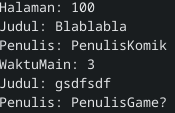
\includegraphics[scale=0.6]{S3.png}
            \end{center}
          \end{multicols}

        \item 

          \begin{multicols}{2}
            \begin{center}
              \lstinputwithcaption{./code/src/soal4/Main.java}{Main.java}
              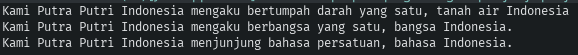
\includegraphics[scale=0.4]{S4.png}
            \end{center}
          \end{multicols}

        \newpage

        \item 

          \begin{multicols}{2}
            \begin{center}

              \lstinputwithcaption{./code/src/soal5/Main.java}{Main.java}

              \columnbreak

              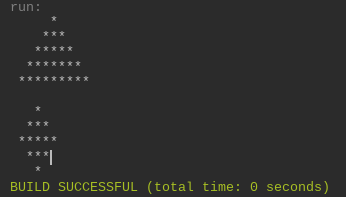
\includegraphics[scale=0.8]{S5.png}

            \end{center}
          \end{multicols}

        \newpage

        \item 

          \begin{multicols}{2}
            \begin{center}

              \lstinputwithcaption{./code/src/soal6/Main.java}{Main.java}

              \columnbreak

              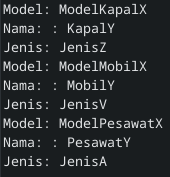
\includegraphics[scale=0.6]{S6.png}

            \end{center}
          \end{multicols}

        \item 

          \begin{multicols}{2}
            \begin{center}

              \lstinputwithcaption{./code/src/soal7/Main.java}{Main.java}

              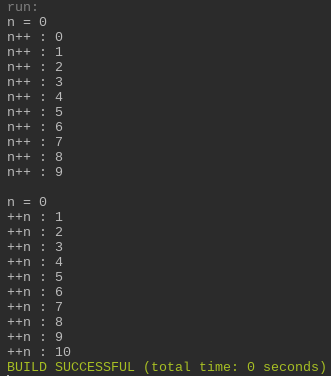
\includegraphics[scale=0.6]{S7.png}

              \columnbreak

              \lstinputwithcaption{./code/src/soal7/ThreadPrint.java}{ThreadPrint.java}


            \end{center}
          \end{multicols}

        \item 

          \begin{multicols}{2}
            \begin{center}

              \lstinputwithcaption{./code/src/soal8/Main.java}{Main.java}

              \columnbreak

              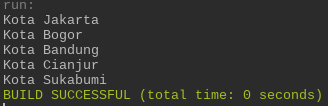
\includegraphics[scale=0.6]{S8.png}

            \end{center}
          \end{multicols}

      \end{enumerate}

    \end{document}
